\noindent
En esta sección desarrollamos el procedimiento práctico para detectar la
retícula de estacionamiento a partir de una imagen de la cámara frontal.
Nos apoyamos en los fundamentos del Marco teórico: Canny y Hough (Sección~\ref{sec:canny-hough}),
la representación de rectas y su intersección en coordenadas homogéneas
(Sección~\ref{sec:rectas-svd}), y los puntos de fuga (Sección~\ref{sec:vanishing-points}).
\noindent
Partimos de una imagen RGB capturada por la cámara frontal. Trabajamos sobre una región de interés (ROI)
definida por debajo del horizonte excluyendo la franja superior para reducir ruido.
Como resultado del procesamiento, obtenemos conjuntos de líneas agrupados según su punto de fuga y un conjunto de esquinas candidatas a vértices de cajón. Dada la naturaleza de la escena, pueden presentarse dificultades como baja textura o contraste, oclusiones y marcas del pavimento degradadas; para mitigarlas, empleamos umbrales ajustables y reintentos por cuadro.

\noindent
Por la proyección perspectiva, las líneas paralelas del mundo se intersectan en la imagen en un punto de fuga
(véase Sección~\ref{sec:vanishing-points} y Fig.~\ref{fig:distorion-teo}).
En nuestro contexto, las marcas de los cajones son aproximadamente paralelas y generan
una retícula de paralelogramos; esto habilita usar la detección de líneas para identificar puntos de fuga
y estimar la posición de la retícula.


\begin{figure}[!ht]
    \centering
    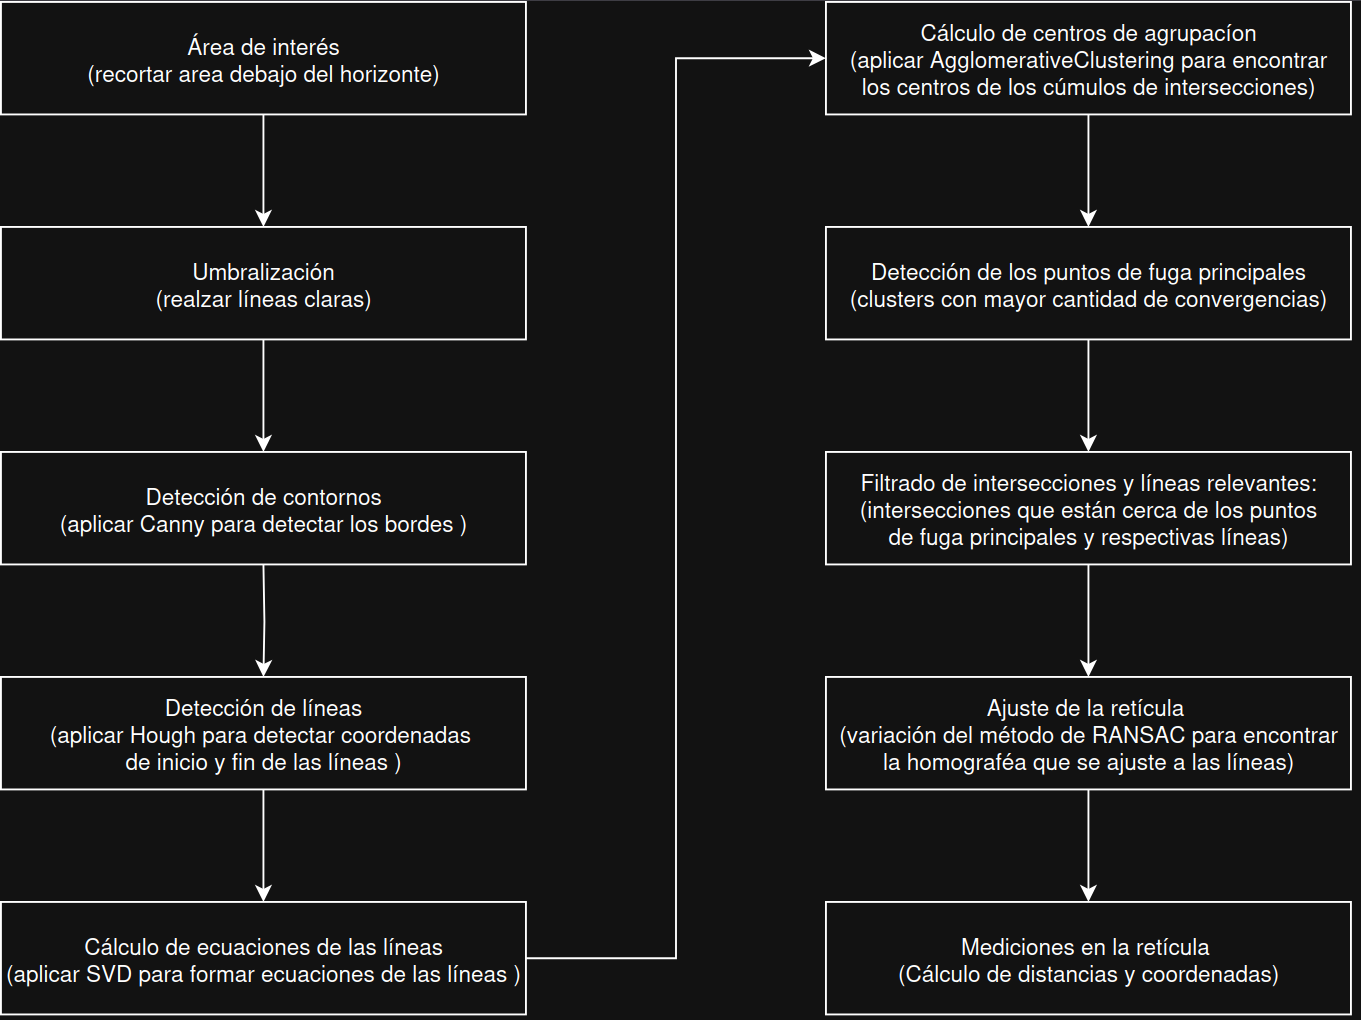
\includegraphics[width=0.8\textwidth]{img/3-metodo/piperline-reticule.png}
    \caption{Diagrama general del pipeline para la detección de la retícula de estacionamiento.}
    \label{fig:reticula-pipeline}
\end{figure}

\noindent
A continuación, desarrollamos cada etapa del diagrama de la Figura~\ref{fig:reticula-pipeline},
centrándonos en el procesamiento de imagen y la extracción de información geométrica relevante con técnicas clásicas de visión computacional.


\subsubsection{Área de interés:}
\noindent
Teniendo en cuenta que la cámara del vehículo se encuentra ubicada en la parte delantera a una altura conocida y en un ángulo paralelo al suelo, el área de interés de la imagen donde se encuentran las líneas de los cajones de estacionamiento quedará siempre por debajo del horizonte de la imagen.
Por lo tanto, se puede eliminar la parte superior de la imagen para
reducir el ruido y mejorar la detección de las líneas, como se muestra en la figura \ref{fig:roi}. \\
\begin{figure}[!ht]
    \centering
    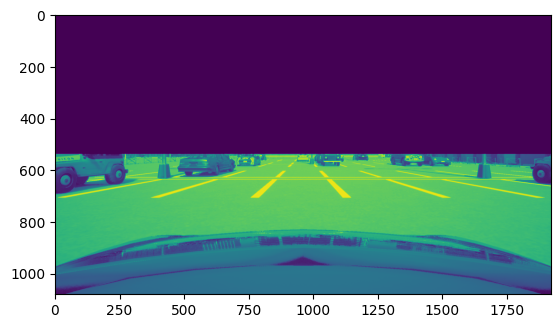
\includegraphics[width=0.9\textwidth]{img/reticule/horizont}
    \caption{Área de interés de la imagen}
    \label{fig:roi}
\end{figure}

\subsubsection{Umbralización:}
\noindent
Al área de interés de la imagen se le aplica una umbralización para realzar las líneas blancas de los cajones de estacionamiento
y eliminar otros elementos no relevantes que puedan interferir en la detección.
En la figura \ref{fig:threshold} se muestra un ejemplo de la imagen umbralizada.
\begin{figure}[!ht]
    \centering
    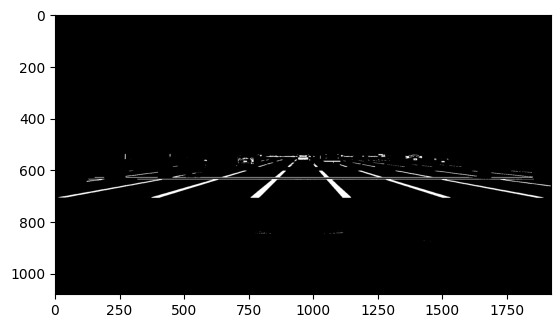
\includegraphics[width=0.9\textwidth]{img/reticule/thresholded}
    \caption{Imagen umbralizada}
    \label{fig:threshold}
\end{figure}

\subsubsection{Detección de contornos (Canny):}
\noindent
Se utiliza el algoritmo de Canny \cite{canny1986edge} (véase Sección~\ref{sec:canny-hough}) para detectar los bordes de las líneas en la imagen umbralizada.
En la figura \ref{fig:edges} se muestra un ejemplo de la imagen con los bordes detectados.
\begin{figure}[!ht]
    \centering
    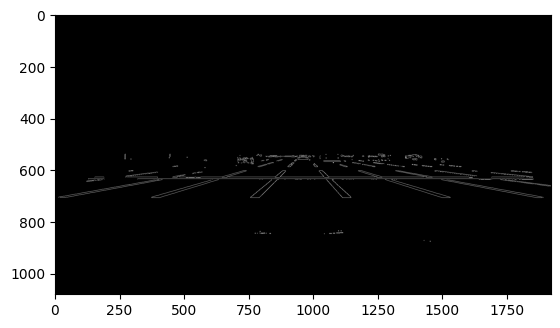
\includegraphics[width=0.9  \textwidth]{img/reticule/canny}
    \caption{Detección de bordes mediante el algoritmo de Canny}
    \label{fig:edges}
\end{figure}

\subsubsection{Detección de líneas (Hough):}
\noindent
Se aplica la transformada de Hough \cite{ballard1981hough} (Sección~\ref{sec:canny-hough}) para detectar las coordenadas de inicio y fin de las líneas en la imagen.
En las figuras \ref{fig:hough} y \ref{fig:lines} se muestran las líneas detectadas sin fondo y sobre la imagen original, respectivamente.
\begin{figure}[!ht]
    \begin{subfigure}{0.5\textwidth}
        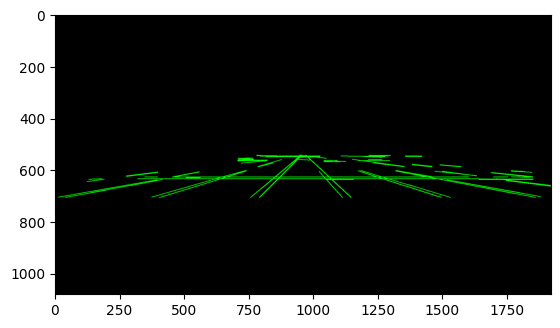
\includegraphics[width=\textwidth]{img/reticule/hough2}
        \caption{Líneas detectadas con la transformada de Hough}
        \label{fig:hough}
    \end{subfigure}
    \begin{subfigure}{0.5\textwidth}
        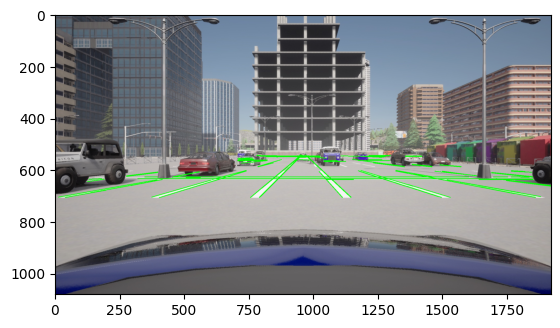
\includegraphics[width=\textwidth]{img/reticule/hough}
        \caption{Líneas detectadas en la imagen original}
        \label{fig:lines}
    \end{subfigure}
\end{figure}

\subsubsection{Representación de las ecuaciones de las líneas:}
\noindent
Una vez obtenidas las coordenadas de inicio y fin de cada línea paralela, se puede utilizar la ecuación general de la recta (véase Sección~\ref{sec:rectas-svd}):
\begin{equation}
    Ax + By + C = 0
\end{equation}
Esta ecuación permite determinar la orientación de cada línea.
Dado que las coordenadas iniciales y finales de cada línea corresponden a los valores de $x$ y $y$, respectivamente,
estas se pueden emplear para formular un sistema de ecuaciones que describa los parámetros de la recta $[A, B, C]$.
Dicho sistema puede representarse de manera matricial como sigue:
\begin{equation}
    \begin{aligned}
        \left[\begin{array}{ccc}
                      x_1 & y_1 & 1 \\
                      x_2 & y_2 & 1
                  \end{array}\right]
        \begin{bmatrix}
            A \\
            B \\
            C
        \end{bmatrix}
        =
        \begin{bmatrix}
            0 \\
            0
        \end{bmatrix}
    \end{aligned}
\end{equation}
\noindent
Esta representación permite calcular de forma precisa los coeficientes de la ecuación de la recta para cada línea detectada,
lo cual es fundamental para analizar su orientación y posición dentro de la retícula de estacionamiento.

\subsubsection{Cálculo de ecuaciones de las líneas (SVD):}
\noindent
Para calcular los coeficientes $[A, B, C]$ de las ecuaciones de las líneas detectadas, se utiliza el concepto de espacio nulo (\emph{null space}) y SVD (Sección~\ref{sec:rectas-svd}).
Este enfoque se basa en el hecho de que cualquier vector en el espacio nulo de una matriz $\mathbf{M}$ satisface la ecuación
\begin{equation}
    \mathbf{Mv} = 0
\end{equation}

\noindent
Cada línea se representa mediante dos puntos $(x_1, y_1)$ y $(x_2, y_2)$. A partir de estas coordenadas homogéneas,
se construye una matriz $\mathbf{M}$ de la forma:
\[
    \mathbf{M} = \begin{bmatrix}
        x_1 & y_1 & 1 \\
        x_2 & y_2 & 1
    \end{bmatrix}
\]
Esta matriz define el sistema de ecuaciones que describe la recta que pasa por los puntos dados.
El espacio nulo de $\mathbf{M}$ corresponde al conjunto de vectores $[A,B,C]$ que satisfacen
\[
    \mathbf{M} \cdot \begin{bmatrix}
        A \\ B \\ C
    \end{bmatrix} = \mathbf{0}.
\]
Se utiliza la Descomposición en Valores Singulares (SVD) \cite{golub2013matrix} para calcular este espacio nulo, ya que es una herramienta robusta y numéricamente estable.
La SVD descompone la matriz \(M\) en tres matrices \(U\), \(S\) y \(V\), donde el espacio nulo de \(M\) se puede obtener a partir de la última columna de la matriz \(V\), que corresponde al vector singular más pequeño (el más cercano a cero).
El vector resultante del espacio nulo se normaliza para que tenga una magnitud manejable.
Esto asegura que los coeficientes \(A\), \(B\) y \(C\) sean comparables entre distintas líneas.

\subsubsection{Cálculo de intersecciones (Clustering):}
\noindent
Una vez que se tienen las ecuaciones de todas las líneas paralelas en el plano de la cámara, se pueden calcular las intersecciones de estas líneas realizando un producto cruz entre las ecuaciones homogéneas [\(A\),\(B\),\(C\)] de todos los pares de líneas.
\noindent
El resultado de este producto cruz es la coordenada homogénea de un punto en el espacio que corresponde a la intersección de las líneas.
Si este punto es finito (cuando la tercera componente no es cero), se puede deshomogeneizar para obtener las coordenadas cartesianas en el plano de la cámara.
En cambio, si el punto es infinito (cuando la tercera componente es muy cercana a cero), significa que las líneas son paralelas y se intersectan en el infinito.

%https://scikit-learn.org/stable/modules/clustering.html#hierarchical-clustering
\noindent
Analizando los puntos de intersección obtenidos que se encuentran en el plano de la cámara, se pueden agrupar para determinar dónde está
concentrada la mayor cantidad de intersecciones.
Este punto de concentración de intersecciones debe corresponder al punto de fuga principal de la retícula de estacionamiento.
En la figura \ref{fig:intersections} se muestra un ejemplo de las intersecciones detectadas en la imagen original,
donde cada color representa un cluster diferente y el símbolo \texttt{+} blanco indica el centro de cada cluster.
\\

\begin{figure}[!ht]
    \centering
    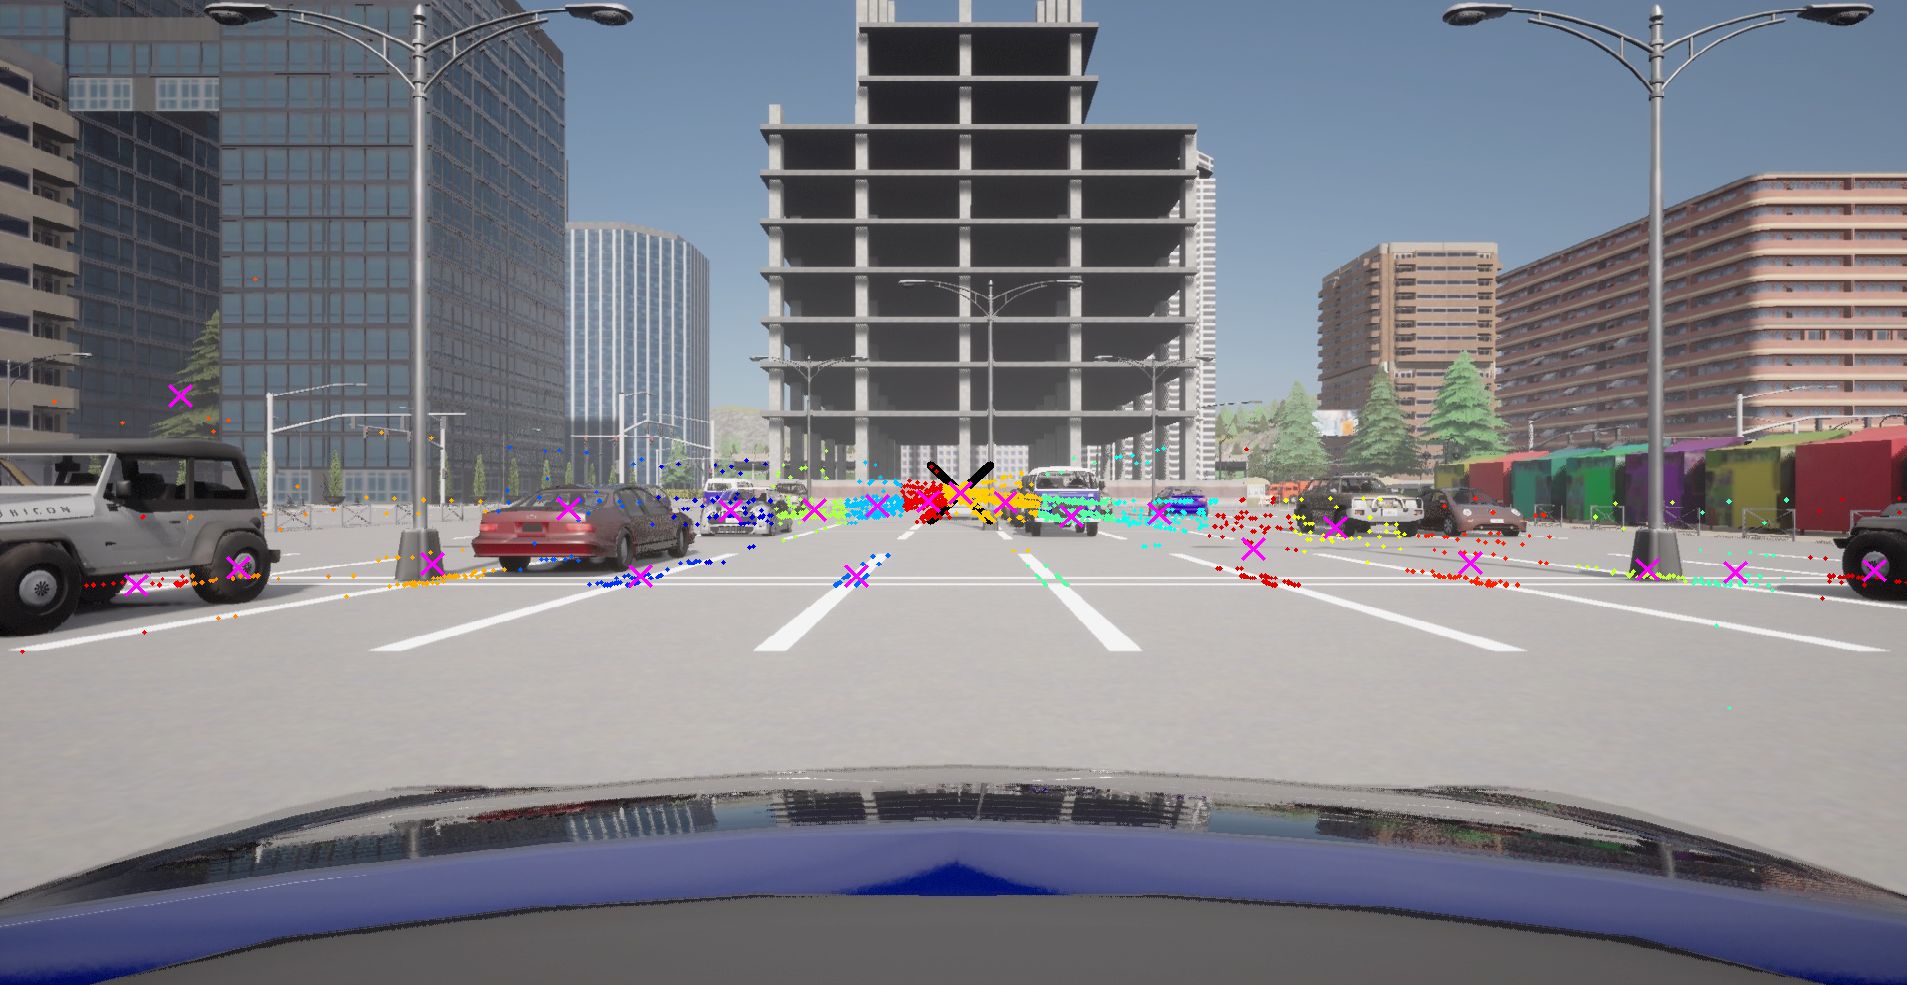
\includegraphics[width=0.9\textwidth]{img/reticule/svd-km}
    \caption{Agrupacion de intersecciones de las líneas detectadas}
    \label{fig:intersections}
\end{figure}
\noindent
Como se discute en la Sección~\ref{sec:intersections-clustering}, para estimar la ubicación de este punto de fuga principal no es necesario tener en cuenta todas las intersecciones detectadas, sino solo aquellas que se encuentran en una zona cercana al horizonte de la imagen (Sección~\ref{sec:vanishing-points}).
Para determinar las intersecciones relevantes cercanas al horizonte, se puede definir un umbral de cercanía en la imagen que se puede ajustar experimentalmente.
Por ejemplo, en la siguiente imagen se muestran las intersecciones detectadas en la imagen original con puntos azules
y las intersecciones relevantes con un umbral de 10 píxeles con puntos amarillos.
En la figura \ref{fig:relevantInter} se muestra el resultado de la selección de las intersecciones relevantes. \\
\begin{figure}[!ht]
    \centering
    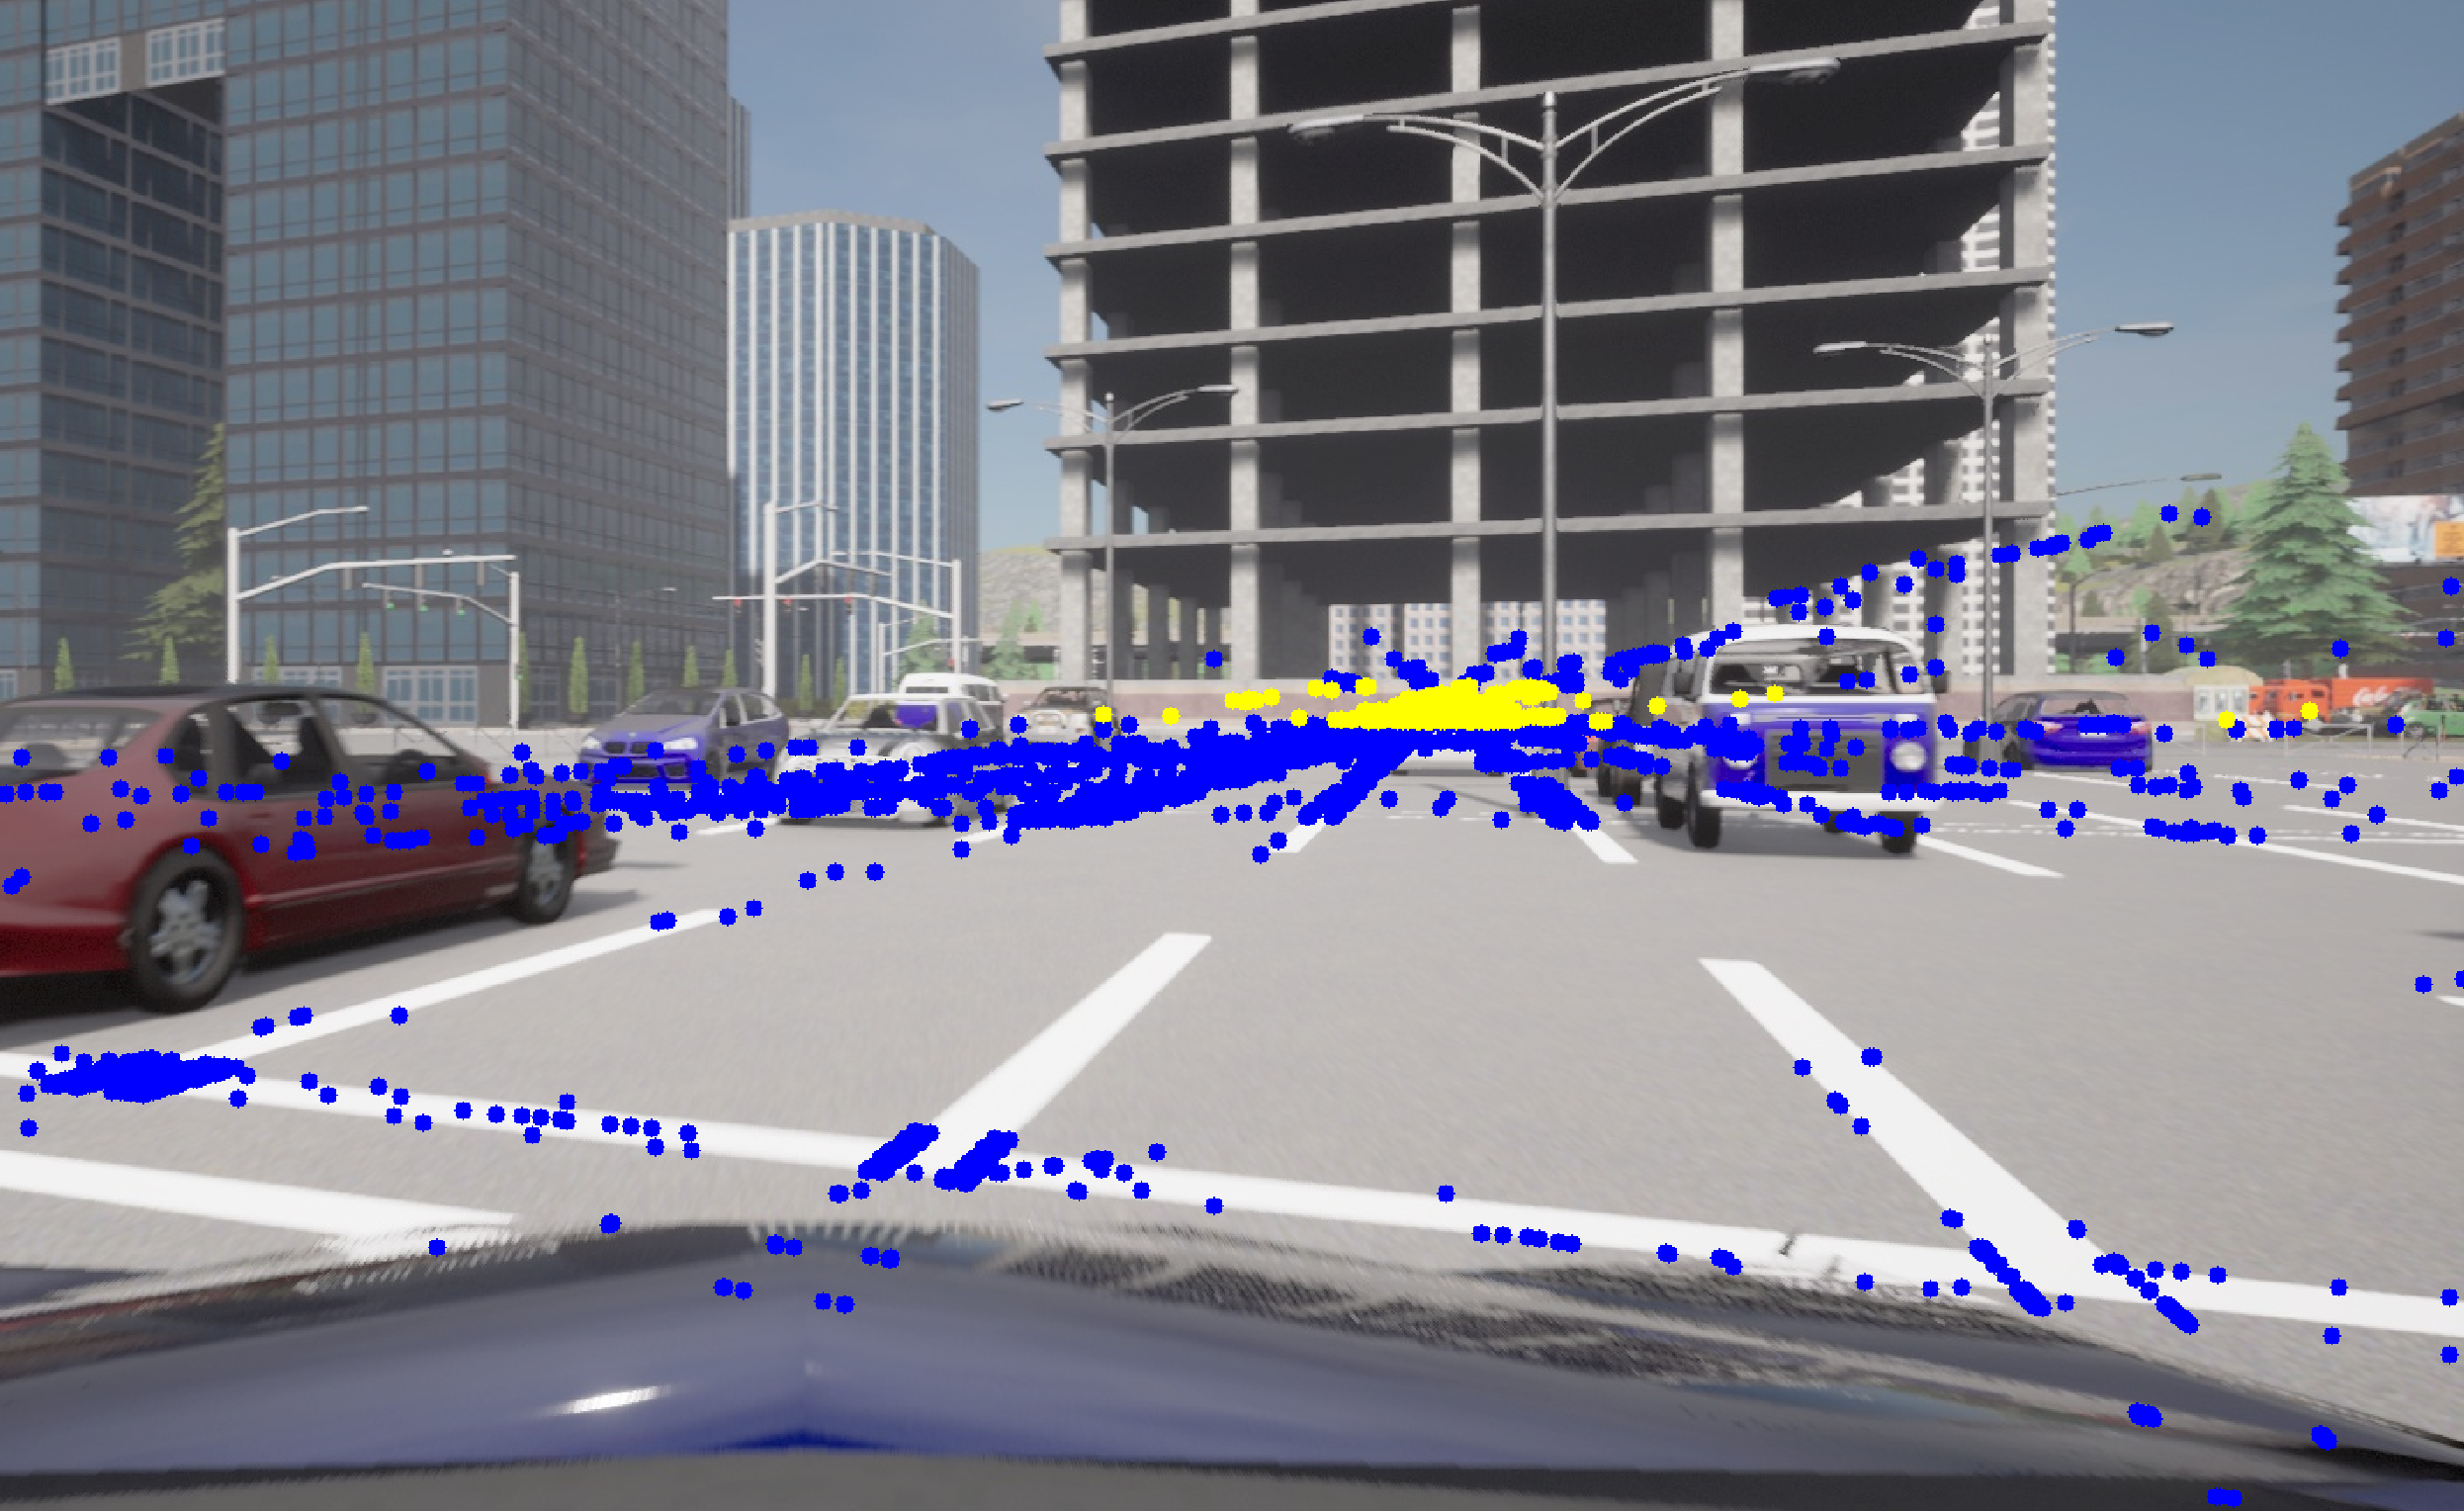
\includegraphics[width=0.9\textwidth]{img/reticule/relevantInter}
    \caption{Intersecciones detectadas en la imagen original}
    \label{fig:relevantInter}
\end{figure}

\noindent
Para agrupar las intersecciones relevantes empleamos \texttt{AgglomerativeClustering} de \texttt{scikit-learn}
(véase Sección~\ref{sec:sklearn-agglomerative}). En nuestra configuración práctica,
dejamos que el algoritmo determine el número de clusters fijando \texttt{distance\_threshold} (distancia máxima entre puntos del mismo
cluster), cuyo valor se ajusta experimentalmente al escenario. A continuación se ilustra el resultado sobre las mismas
intersecciones relevantes del ejemplo anterior: se forman 3 clusters (colores distintos) y se marca con \texttt{+} blanco el centroide de cada uno
(Fig.~\ref{fig:clusters}).
\begin{figure}[!ht]
    \centering
    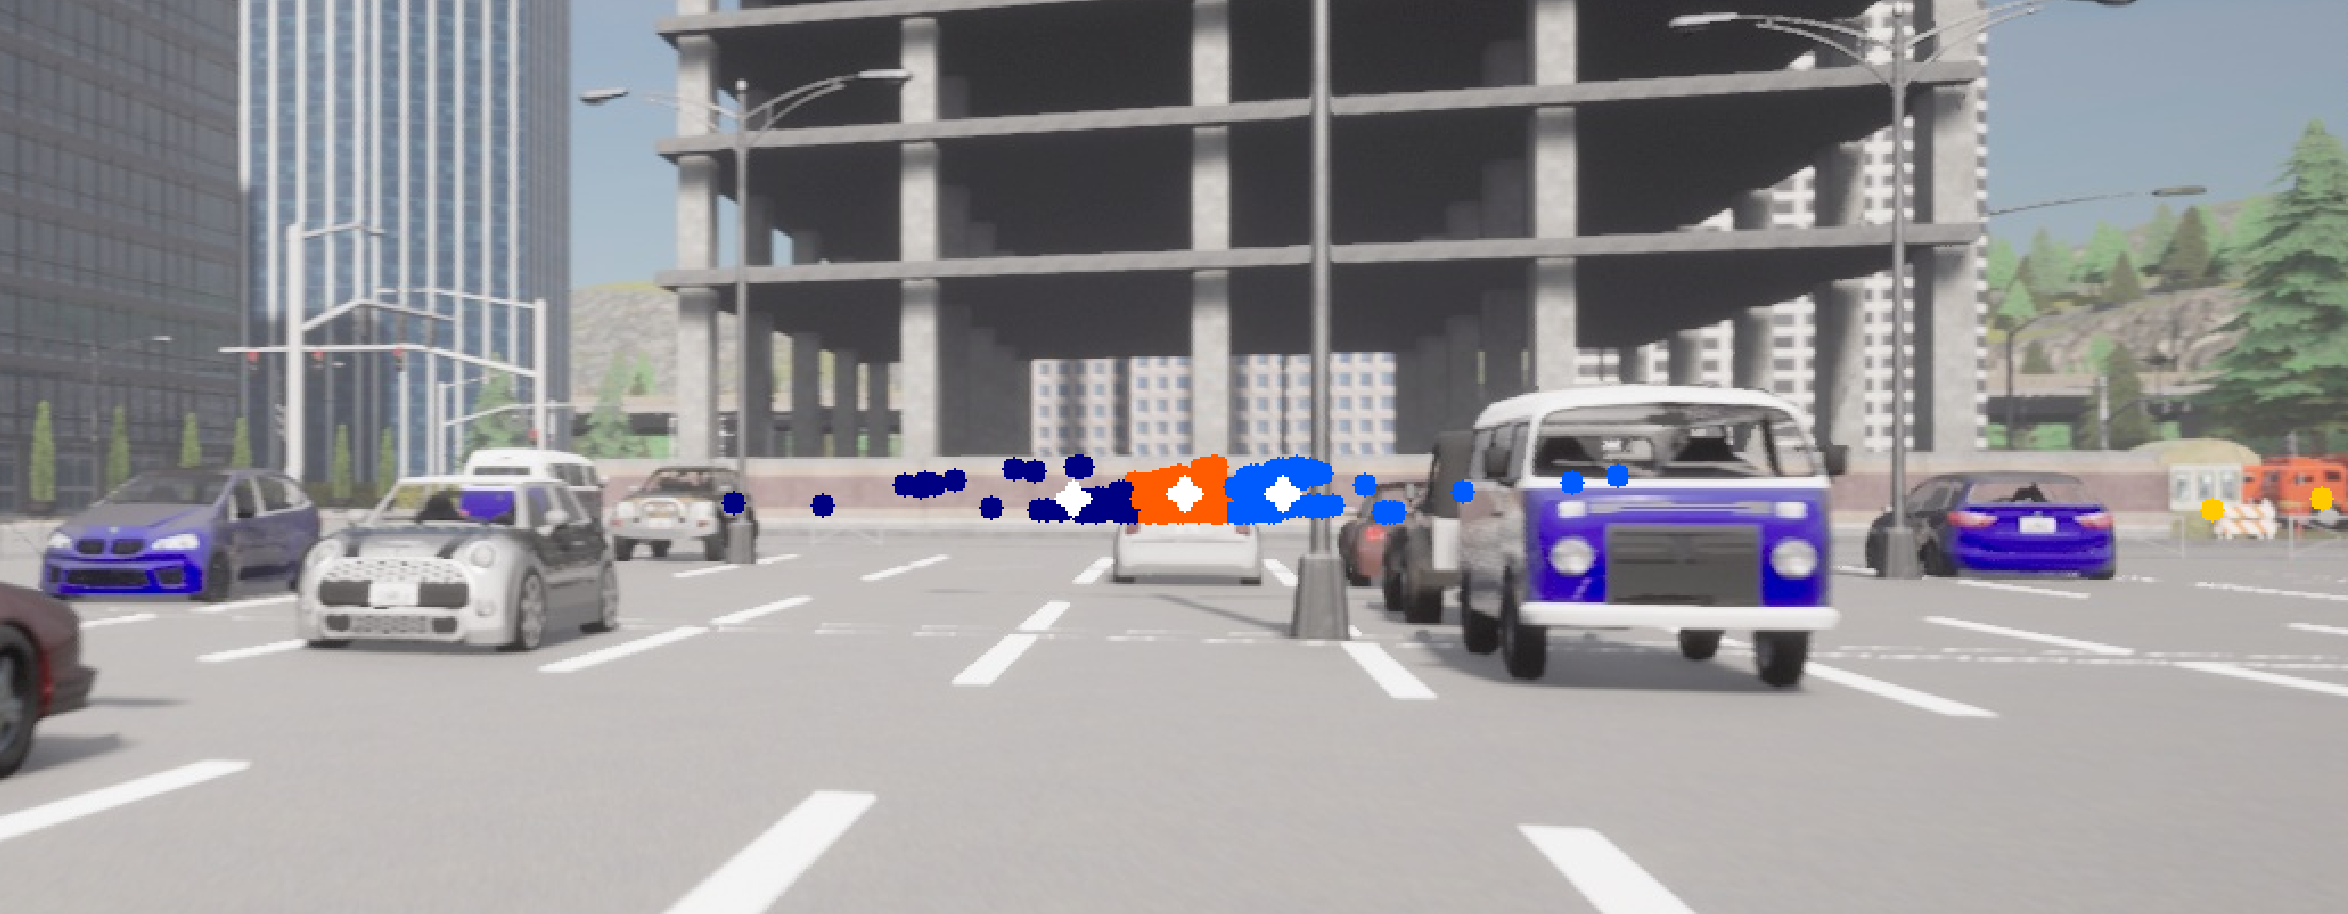
\includegraphics[width=0.9\textwidth]{img/reticule/AgglomerativeClustering}
    \caption{Intersecciones agrupadas en clusters}
    \label{fig:clusters}
\end{figure}



\subsubsection{Selección del punto de fuga principal:}
\noindent
Para estimar la posición del punto de fuga principal, se puede seleccionar el cluster con mayor cantidad de intersecciones y
utilizar las líneas que generaron estos puntos para calcular la intersección de estas líneas.
La intersección de $n$ líneas (bajo un criterio de mínimos cuadrados) está dada por
el eigenvector asociado al eigenvalor más pequeño de la matriz $M$, donde:
\[
    M = \sum_{i=1}^{n} w_i l_i l_i^T
\]
Aquí, $w_i$ es un peso asociado a la línea $l_i$ y $l_i$ es la representación homogénea de la línea $i$ \cite{kanatani1998statistical}.
De esta forma, podemos conocer la posición del punto de fuga principal en el plano de la cámara.
En la figura \ref{fig:vanishingPoint} se muestra el resultado de esta estimación utilizando las líneas del cluster más grande, donde se
representa el punto de fuga principal con un símbolo \texttt{+} amarillo.
\begin{figure}[!ht]
    \centering
    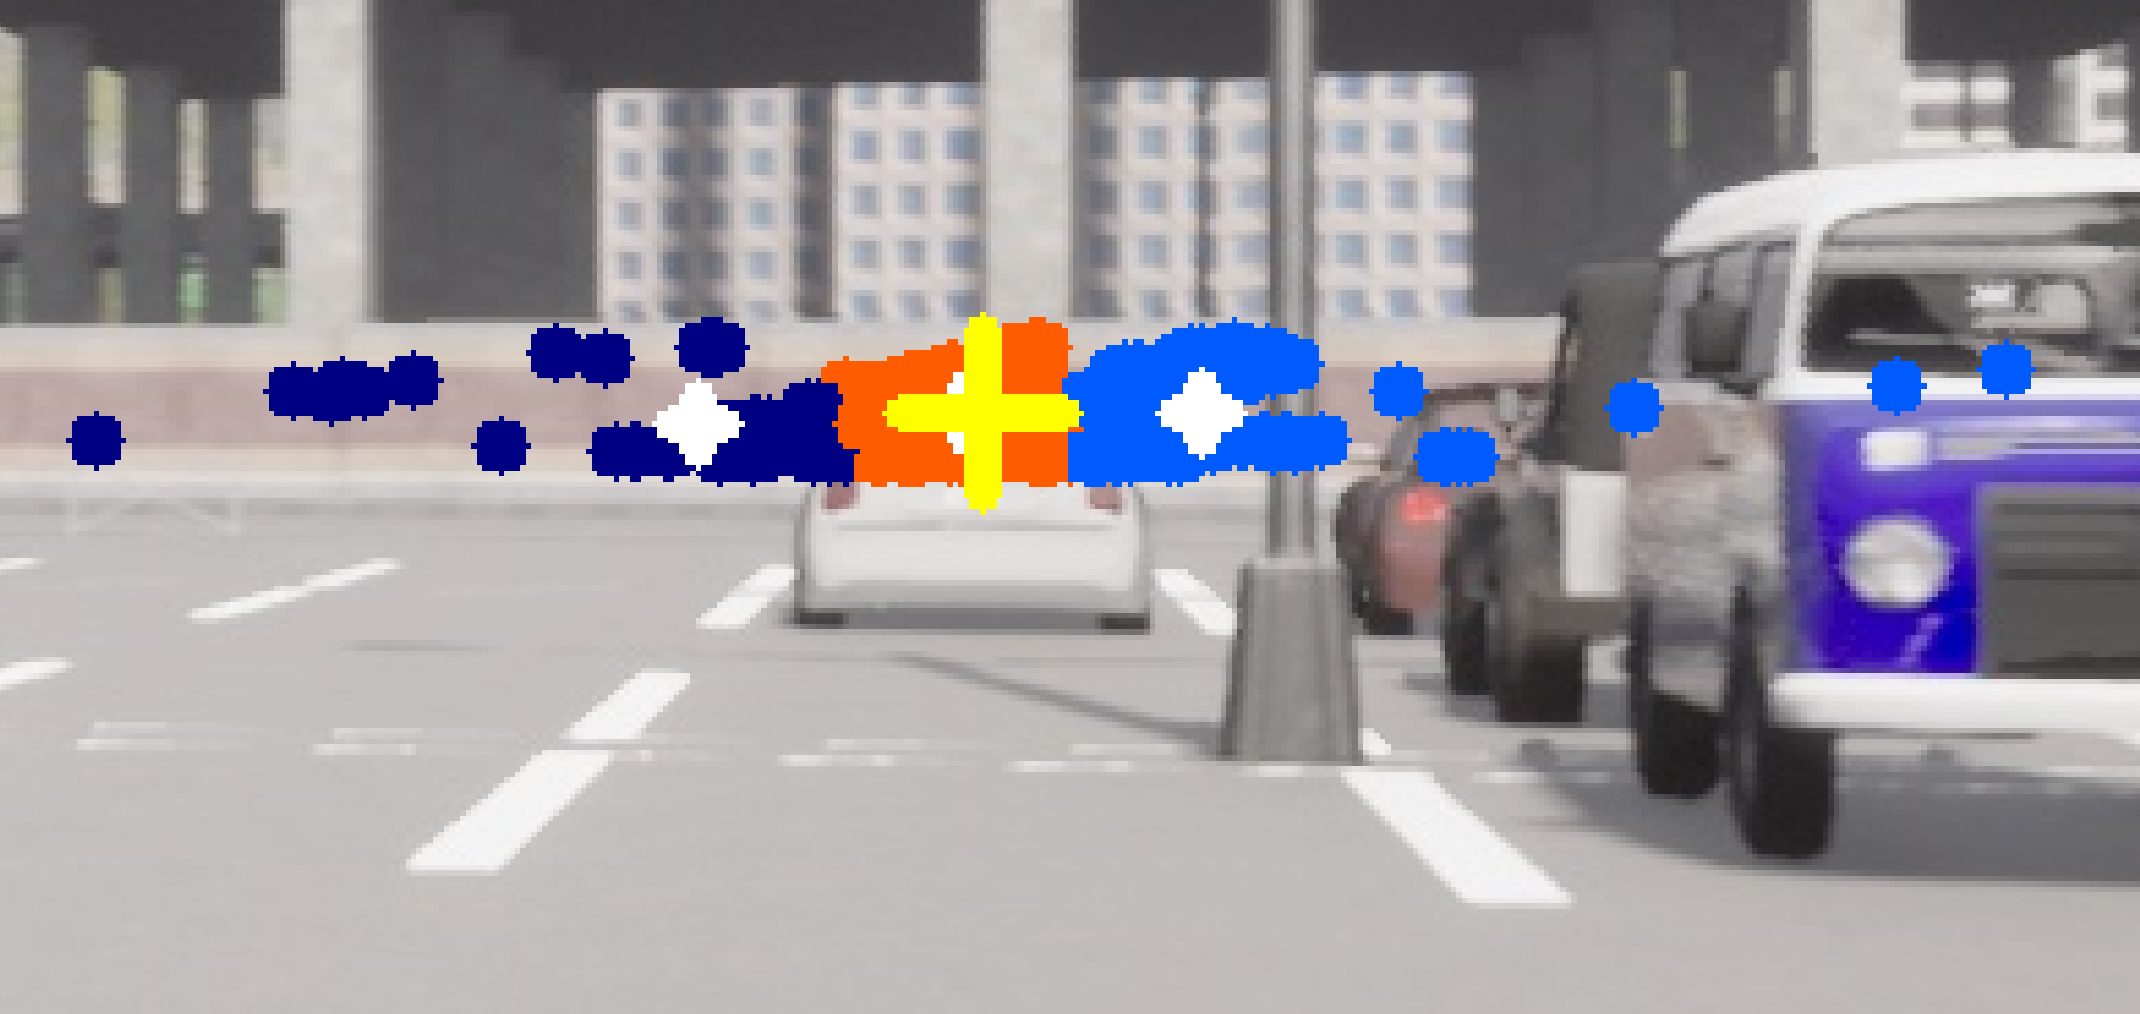
\includegraphics[width=0.9\textwidth]{img/reticule/vanishingPoint}
    \caption{Punto de fuga principal estimado}
    \label{fig:vanishingPoint}
\end{figure}

\subsubsection{Selección del 2do punto de fuga principal:}
Pendiente de redacción.

\subsubsection{Filtrado de intersecciones y líneas relevantes:}
\noindent
Una vez que se han identificado los puntos de fuga principales, se puede proceder a filtrar las intersecciones y las líneas que son
relevantes para la retícula de estacionamiento.
Primero, se filtran las intersecciones que están cerca de los puntos de fuga principales, utilizando un umbral de distancia que se puede ajustar experimentalmente.
Luego, se filtran las líneas que pasan por estas intersecciones relevantes.
Este proceso ayuda a eliminar el ruido y las líneas que no contribuyen a la formación de la retícula de estacionamiento.


\subsubsection{Experimentación y ajuste de parámetros}
\noindent
La herramienta de experimentación y la lista completa de parámetros ajustables se describen en el Marco teórico
(Sección~\ref{sec:experimentation-tool}). Aquí nos limitamos a referenciarla, pues sirve como apoyo para calibrar
los umbrales y validaciones usados a lo largo del pipeline práctico.

\subsubsection{Mediciones en la retícula detectada:}
Pendiente de redacción.
